%---------------------%
%     Use of Scrum     %
%-------------------- %
\subsection{Use of Scrum}
\begin{frame}{Development Method}
  What is Scrum?
  \linespace

  \begin{itemize}
  \item Framework used to address complex adaptive problems
    \begin{itemize}
    \item Ensures products of highest possible value
    \end{itemize}
  \end{itemize}

	\begin{figure}
		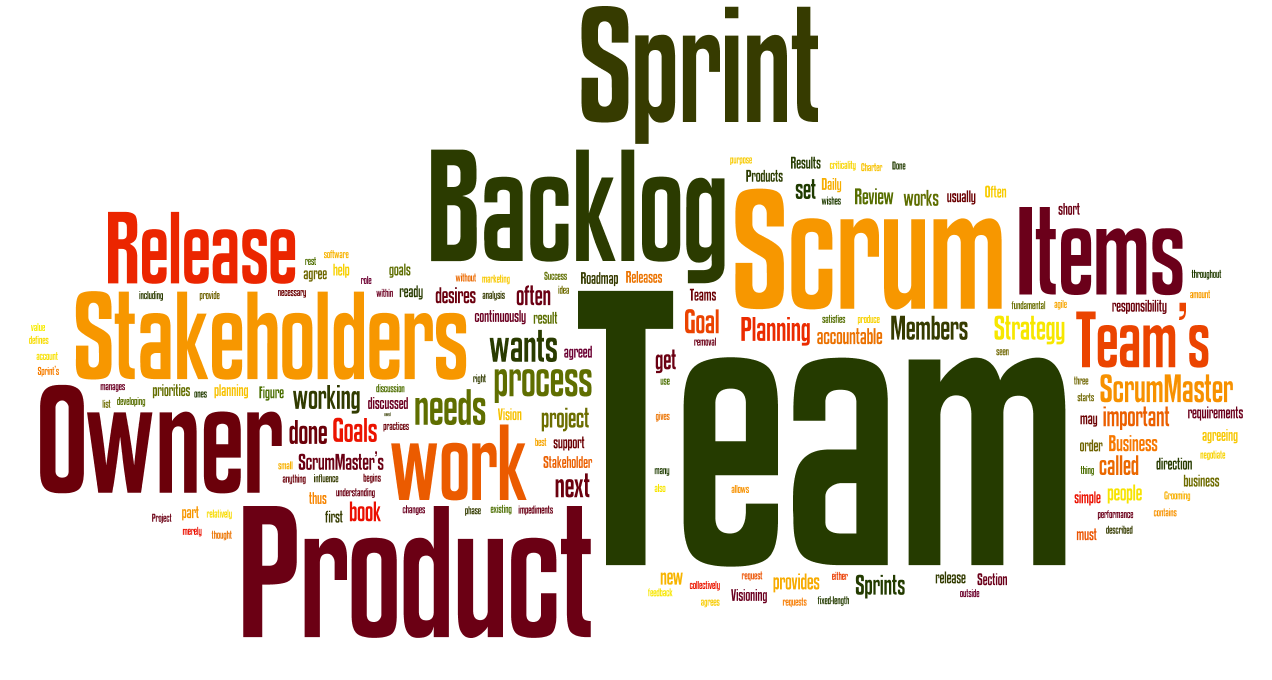
\includegraphics[width=1\textwidth]{slides/agile-glossary.png}
	%	\caption{http://www.scrumhint.com/wp-content/uploads/2013/05/agile-glossary.png}
	\end{figure}
\end{frame}

\begin{frame}{Multi-Project Scrum usage}
  \begin{columns}
  		\begin{column}{0.5\textwidth}
  			Actual Use:
  			\linespace
  			\begin{itemize}
  				\item Point 1
  			\end{itemize}
  		\end{column}
  		\pause
  		\begin{column}{0.5\textwidth}
  			Optimal Use:
  			\linespace
  			\begin{itemize}
  				\item Point 1
  			\end{itemize}
  		\end{column}
  \end{columns}
\end{frame}

\begin{frame}{Group Scrum usage}
  \begin{columns}
  		\begin{column}{0.5\textwidth}
  			Intentions to form a Scrum of Scrums, to:
  			\linespace
  			\begin{itemize}
  				\item Syncronize progress with multi-project Scrum
  				\item Need more points here...
  			\end{itemize}
  		\end{column}
  		\pause
  		\begin{column}{0.5\textwidth}
  			Did not work as expected:
  			\linespace
  			\begin{itemize}
  				\item Failed to sustain to Scrum Events
    				\begin{itemize}
    				\item Sprint Planning
    				\item Daily Scrum
    				\item Sprint Review
    				\end{itemize}
    		  \item Did not utilize Scrum Roles
      		  \begin{itemize}
      		  \item Product Owner
      		  \item Scrum Master
      		  \end{itemize}
      		\item Scrum Retrospective
  			\end{itemize}
  		\end{column}
  \end{columns}
\end{frame}

\begin{frame}{Reflecting on Groups usage of Scrum}
  
  \linespace
  \begin{itemize}
  \item Roles
    \begin{itemize}
    \item Scrum Master
    \item Product Owner
      \begin{itemize}
      \item A client?
      \end{itemize}
    \end{itemize}
  \item Scrum Board vs. Redmine
  \item Keep track of pace
    \begin{itemize}
    \item Burn-down chart
    \end{itemize}
  \end{itemize}
\end{frame}

%--------------------------------------------------
%     OOD
%--------------------------------------------------
\subsection{Object Oriented Design}
\begin{frame}{Unstructured approach}
	\begin{itemize}
		\item<1> Taking over an existing project
		\item<2> Refactoring vs. re-writing
		\item<3> Ad-hoc design
  		\begin{itemize}
  		\item Case: View Holder pattern Android best-practice
  		\end{itemize}
		\begin{center}
		\includegraphics<2>[width=0.8\textheight]{slides/swengineer}
		\end{center}
	\end{itemize}
\end{frame}

\begin{frame}{Design Patterns}
Start med ``How to improve?''
\end{frame}